\section{Navigation} \label{s:navi}
To make it possible to navigate a drone indoors, there are obstacles which are needed to be considered. There are two types of obstacles, permanent and temporary. The permanent obstacles can be the following; walls, ceiling, doors, windows and furniture. Temporary obstacles are objects like people or things placed in the path temporarily. This means it is necessary to avoid any collision with any humans and other objects, that can occur suddenly in front of the drone. The drone should be capable of detecting those obstacles. 
\newline

The drone needs to have different sensors to detect the obstacles. Some sensors that can be used in these situations are distance sensors. The drone need a minimum number of distance sensors to cover all the surroundings, as shown on figure \ref{fig:drone_sensor}.
\begin{figure}[H]
    \centering
    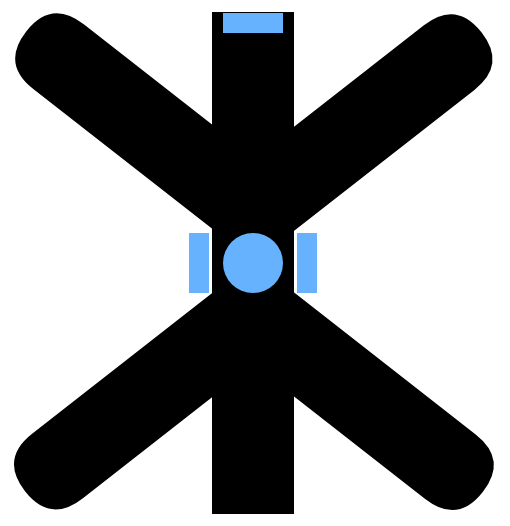
\includegraphics[width=0.3\textwidth]{figures/Navigation/DroneIR.png}
    \caption{Illustration of where the sensors can be placed on the drone.}
    \label{fig:drone_sensor}
\end{figure}
There are different sensors there can use to navigating a drone indoors. Sensors like Infra Red, Ultrasonic and Vision will be explained in the following sections.

\subsection*{Infra Red sensor}
One of the possible sensors are IR sensors, which is used in different devices such as laser distance meter. An IR sensor consists of an IR transmitter and an IR receiver. 
The IR sensor works by the transmitter flashing an infrared light out, when the light hits a surface, the light gets reflected back to the sensor's receiver. The distance then gets calculated from the time of flight, this is the time from when the light is flashed and to the sensor registers it again.


There are some disadvantage with IR sensors, which can be light distortion and different materials could reflect the light differently, this could interfere with the sensor measuring.
\newline
Ultrasonic sensors works the same as the IR sensors, the only difference is it uses ultra sound instead of infra red light.

\subsection*{Vision sensor}\label{ss:camera_pa}
Vision sensors consist of an image sensor that take images of their field of vision. These images can then be processed by a computer vision algorithm, to classify objects and avoid them.

The images can both be normal images captured with a normal image sensor, or the system could use Time of Flight depth image sensors, and get even more information for object classification

The main disadvantage of such a system, is the high complexity of both the hardware and software required. Such a vision system would require power full hardware to do real time image recognition, and the complexity of the software is outside the scope of this project.

\subsection*{Conclusion}
From the problem analysis it can be concluded that, a time-of-flight sensor will suit this project best. It is simple to implement and a good reliable sensor type. The only problem with it, is the time it takes before having the distance. To prevent this a good sampling time is needed, to make it possible to be used for checking distances to a surface.
\newline
To make the sampling time as small as possible an IR sensor have been chosen, these type of sensors have a much faster sampling time then a ultrasonic sensor.






